\section*{Problem Statement}
The objective of this problem is to analyze the error in approximating the exponential function $f(x) = e^x$ using Lagrange interpolation. Specifically, we evaluate and plot the theoretical error bound over a given set of interpolation nodes.

\begin{quote}
  \textbf{NOTE}: The code can be accessed using this link: \href{https://raw.githubusercontent.com/HavokSahil/computational-techniques-assignments/refs/heads/main/assignment3/a3.m}{MATLAB}, \href{https://raw.githubusercontent.com/HavokSahil/computational-techniques-assignments/refs/heads/main/assignment3/a3.jl}{Julia}.
\end{quote}

\section*{Methodology}
The interpolation error for a function $f(x)$ using $n$ nodes is given by:
\[
  R_n(x) = \frac{f^{(n+1)}(\xi)}{(n+1)!} \prod_{i=0}^{n} (x - x_i), \quad \xi \in [\min(X), \max(X)].
\]

For $f(x) = e^x$, all derivatives are $f^{(k)}(x) = e^x$. Therefore, an upper bound for the error can be expressed as:
\[
  |R_n(x)| \leq \frac{e^{\max(X)}}{(n+1)!} \prod_{i=0}^{n} |x - x_i|.
\]

Steps:
\begin{enumerate}
  \item Define interpolation nodes $X = \{0.1, 0.2, 0.3, 0.4, 0.5, 0.6\}$.
  \item Implement a function to compute the error bound $err\_bound(X, x)$.
  \item Sample points $x \in [0.1, 0.6]$ with step $0.01$.
  \item For each sampled point, compute the error bound.
  \item Plot the error bound as a function of $x$.
\end{enumerate}

\section*{Results}
The chosen interpolation nodes are:
\[
X = \{0.1,\,0.2,\,0.3,\,0.4,\,0.5,\,0.6\}.
\]

The theoretical error bound was evaluated for points in the interval $[0.1, 0.6]$. The resulting plot shows how the error grows as $x$ moves away from the interpolation nodes, with the error minimized near the nodes themselves.

\begin{figure}[h!]
  \centering
  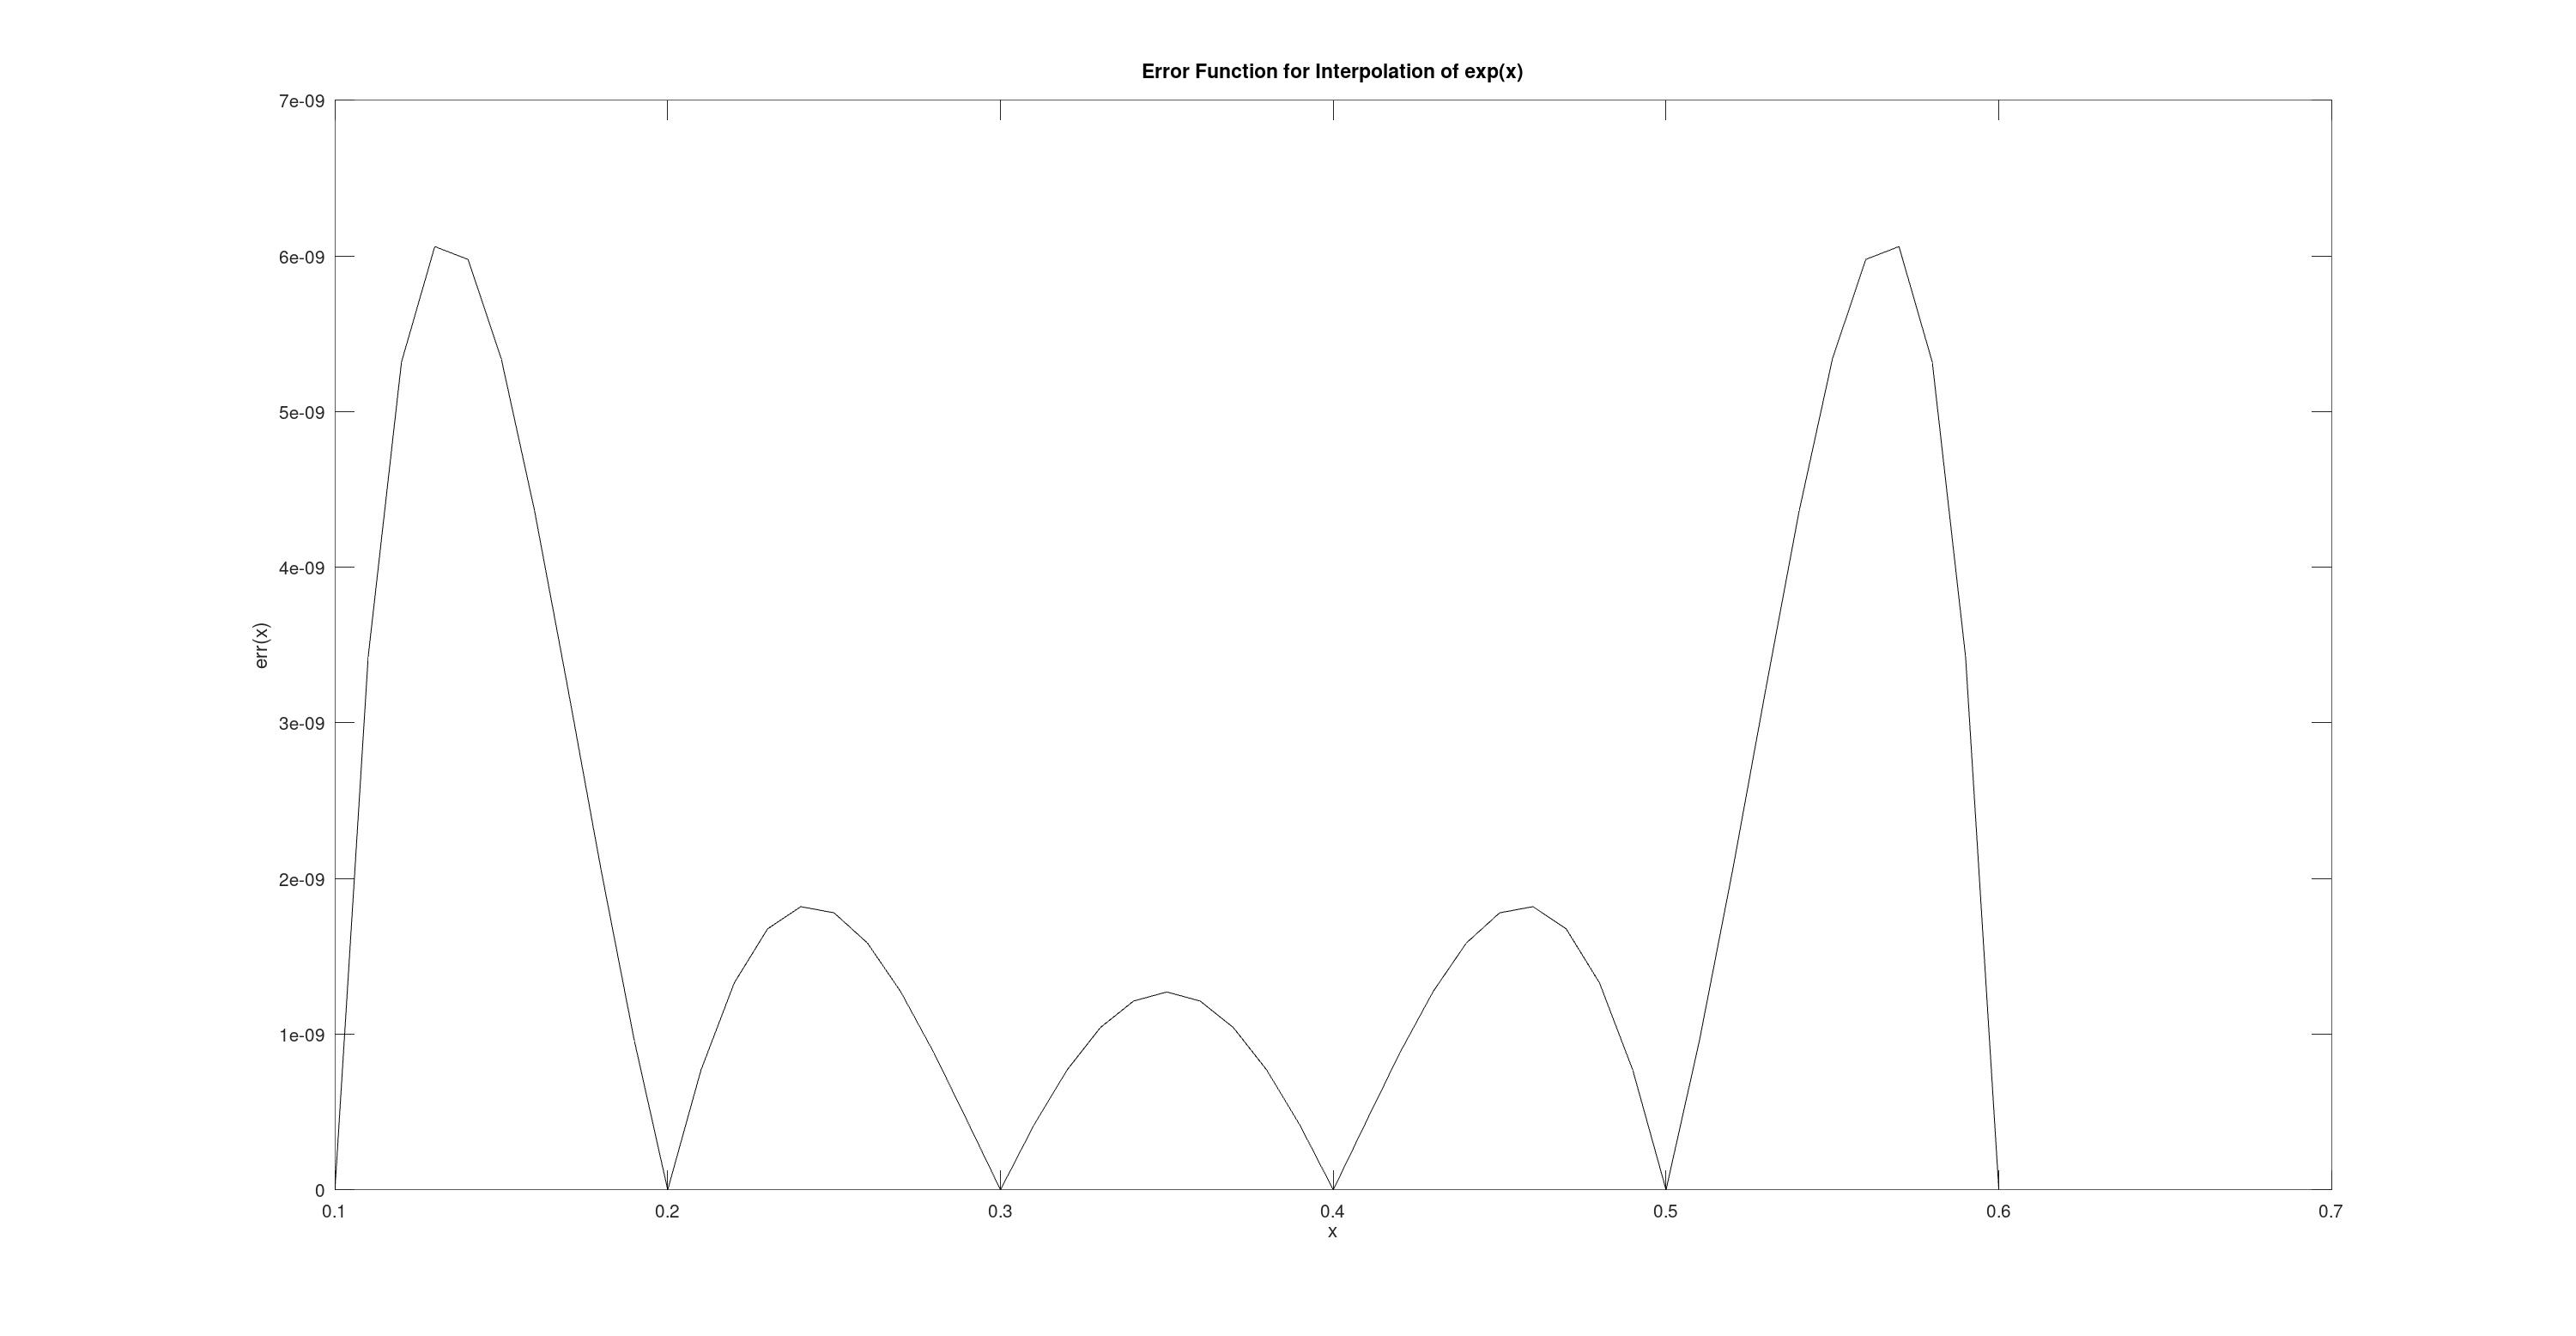
\includegraphics[width=1.0\textwidth]{a3.jpg}
  \caption{Error Bound Plot for values of x}
  \label{fig:a3}
\end{figure}


\section*{Conclusion}
The error bound for Lagrange interpolation of $e^x$ was computed and plotted. The bound illustrates two key properties:
\begin{itemize}
  \item The error vanishes at interpolation nodes $x_i$ since the product term contains $(x - x_i)$.
  \item The error increases between nodes, with larger deviation near the ends of the interval.
\end{itemize}

This confirms the theoretical behavior of interpolation errors and highlights that interpolation accuracy depends strongly on both the function’s smoothness and the placement of interpolation nodes.
